\documentclass{article}
\usepackage{graphicx}
\usepackage{amsmath}
\usepackage{booktabs}
\usepackage{siunitx}
\usepackage{float}
\usepackage{listings}
\usepackage{xcolor}
\usepackage[margin=1in]{geometry}

\lstset{
  language=Matlab,
  basicstyle=\small\ttfamily,
  keywordstyle=\color{blue},
  commentstyle=\color{green!50!black},
  numbers=left,
  numberstyle=\tiny\color{gray},
  frame=single,
  breaklines=true
}

\title{Homework 2 - ET4369 Nyquist Rate Data Converters}
\author{Daniel Tyukov \\ Student Number: 5714699 \\ Electrical Engineering, TU Delft}
\date{March 2026}

\begin{document}

\maketitle
\tableofcontents
\newpage

%% ============================================================
%% PROBLEM 1
%% ============================================================
\section{Reconstruction (ZOH)}

\textbf{Given:} Discrete-time signal $x(n)$ with $f_s = 125$\,MHz, converted to continuous time using zero-order-hold (ZOH) pulses.

\subsection{Part (a): Amplitude Envelopes}

For a rectangular hold pulse of width $T_p$, the ZOH output spectrum is the sampled spectrum multiplied by the amplitude envelope:
\begin{equation}
    |H_p(f)| = \frac{T_p}{T_s} \cdot |\operatorname{sinc}(f \cdot T_p)| = \frac{T_p}{T_s} \cdot \left|\frac{\sin(\pi f T_p)}{\pi f T_p}\right|
\end{equation}
where $T_s = 1/f_s = 8$\,ns.

The three hold pulse widths and their DC gains:

\begin{table}[H]
\centering
\begin{tabular}{@{}ccc@{}}
\toprule
$T_p$ & $T_p/T_s$ & Description \\
\midrule
2\,ns & 0.25 & Short RZ pulse ($\frac{1}{4}$ of period) \\
4\,ns & 0.50 & Half-period RZ pulse \\
8\,ns & 1.00 & Full-period NRZ ($T_p = T_s$) \\
\bottomrule
\end{tabular}
\end{table}

\begin{figure}[H]
    \centering
    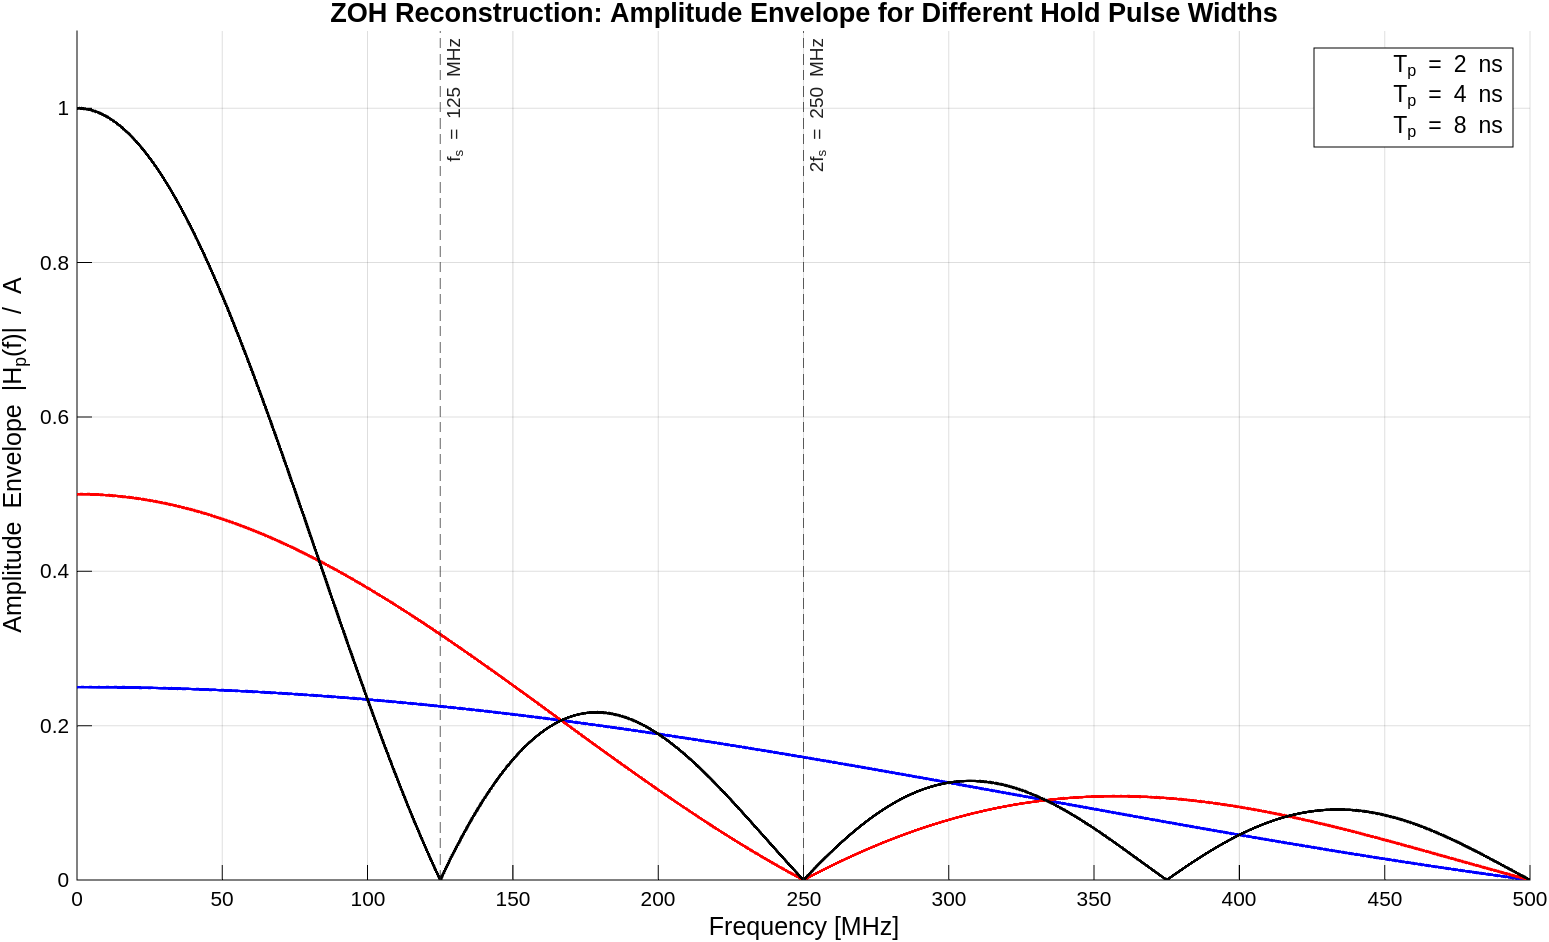
\includegraphics[width=0.9\textwidth]{p1a_amplitude_envelopes.png}
    \caption{ZOH amplitude envelopes for three hold pulse widths.}
    \label{fig:p1a}
\end{figure}

\textbf{Observations:}
\begin{itemize}
    \item The 8\,ns (NRZ) case has the highest DC gain (1.0) but the steepest sinc roll-off, with a null at $f_s = 125$\,MHz. This provides the strongest suppression of spectral images near $f_s$, but also the most in-band signal droop.
    \item The 2\,ns case has the flattest response (first null at $1/T_p = 500$\,MHz), but only 0.25 DC gain. Images are poorly suppressed.
    \item The 4\,ns case is intermediate: first null at 250\,MHz, DC gain of 0.5.
\end{itemize}

\subsection{Part (b): Output Tones for 8\,ns Hold, 30\,MHz Sine Input}

With $T_p = 8$\,ns (NRZ, $T_p = T_s$), $f_\text{in} = 30$\,MHz, and $f_s = 125$\,MHz, the sampled signal contains spectral images at $f = f_\text{in} + k \cdot f_s$ for all integers $k$. Folding to positive frequencies, the tones up to 250\,MHz are:

\begin{table}[H]
\centering
\begin{tabular}{@{}cccccc@{}}
\toprule
Tone & Frequency & Origin & $f \cdot T_p$ & $\operatorname{sinc}(f \cdot T_p)$ & Amplitude$/A$ \\
\midrule
1 & 30\,MHz  & $f_\text{in}$        & 0.24 & 0.9079 & \textbf{0.9079} \\
2 & 95\,MHz  & $f_s - f_\text{in}$  & 0.76 & 0.2867 & \textbf{0.2867} \\
3 & 155\,MHz & $f_s + f_\text{in}$  & 1.24 & 0.1757 & \textbf{0.1757} \\
4 & 220\,MHz & $2f_s - f_\text{in}$ & 1.76 & 0.1238 & \textbf{0.1238} \\
\bottomrule
\end{tabular}
\caption{Output tones for 8\,ns NRZ hold with 30\,MHz sine input.}
\label{tab:tones}
\end{table}

Each tone's amplitude (normalized to $A$) equals the sinc envelope evaluated at that frequency:
\begin{equation}
    \text{Amplitude}(f) = |\operatorname{sinc}(f \cdot T_p)| = \frac{|\sin(\pi f T_p)|}{\pi f T_p}
\end{equation}
since $T_p / T_s = 1$ for the NRZ case.

\begin{figure}[H]
    \centering
    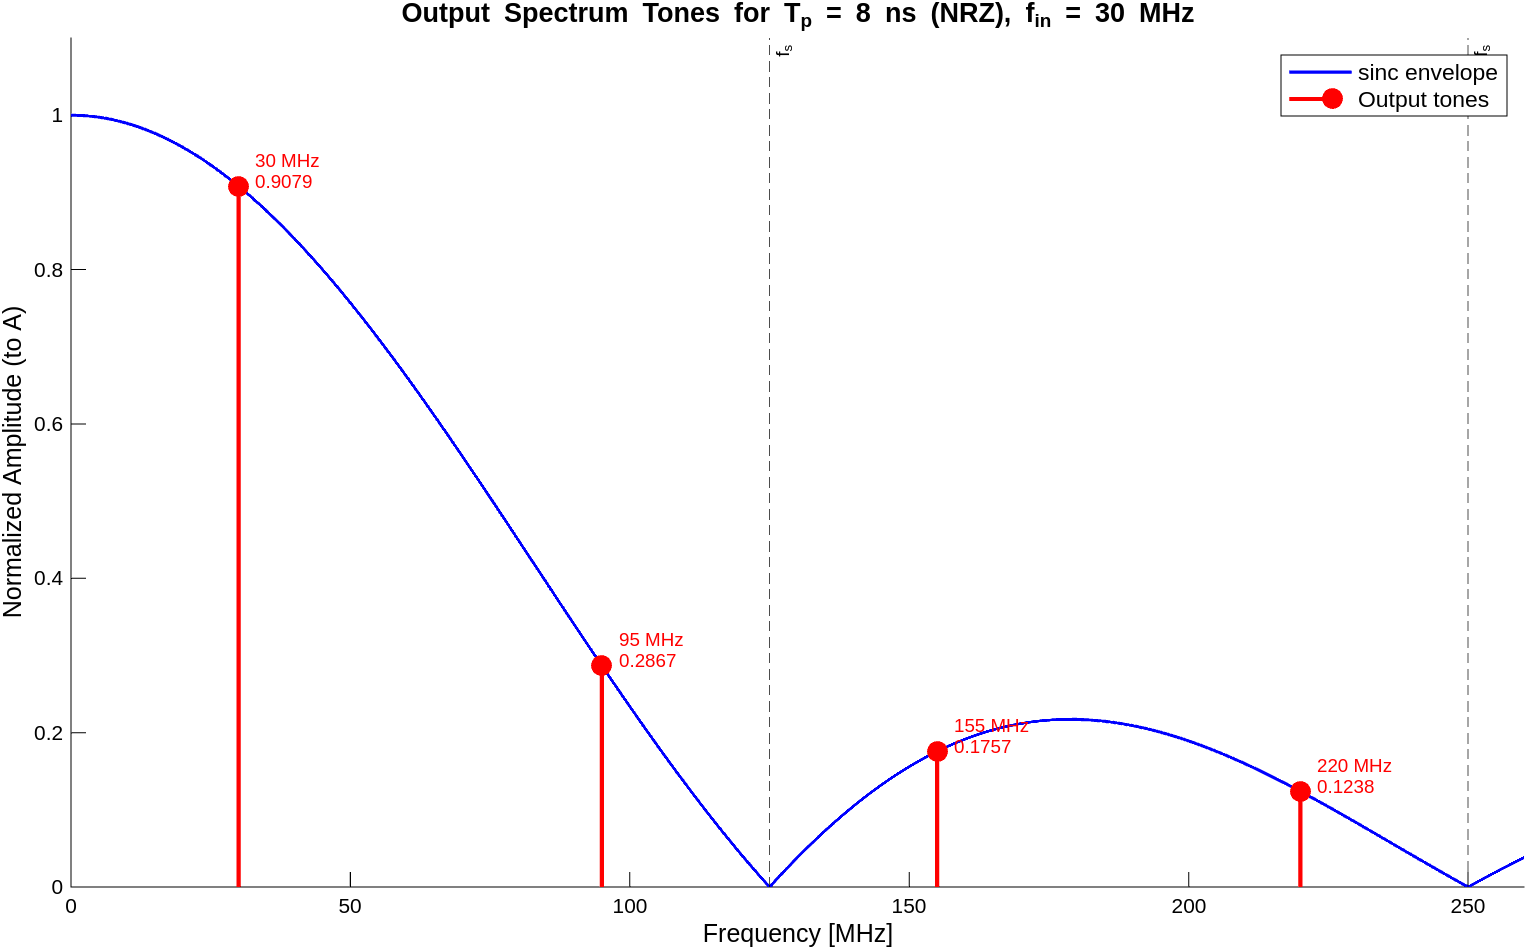
\includegraphics[width=0.9\textwidth]{p1b_output_tones.png}
    \caption{Output spectrum tones for $T_p = 8$\,ns (NRZ), $f_\text{in} = 30$\,MHz.}
    \label{fig:p1b}
\end{figure}

\textbf{Observations:}
\begin{itemize}
    \item The fundamental at 30\,MHz suffers about 9.2\% attenuation (sinc droop) --- from $A$ to $0.908A$.
    \item The first image at 95\,MHz ($= f_s - f_\text{in}$) is the strongest unwanted tone at $0.287A$ ($-10.0$\,dB relative to the fundamental).
    \item Images at 155\,MHz and 220\,MHz are further suppressed to $0.176A$ and $0.124A$ respectively.
    \item A reconstruction filter is needed to suppress these image tones and optionally compensate the sinc droop.
\end{itemize}

%% ============================================================
%% PROBLEM 2
%% ============================================================
\section{Segmented DAC Design --- Paper Review}

\textbf{Paper:} C.-H.~Lin and B.~Bult, ``A 10-b, 500-MSample/s CMOS DAC in 0.6\,mm\textsuperscript{2},'' \textit{IEEE J.\ Solid-State Circuits}, vol.~33, no.~12, pp.~1948--1958, Dec.~1998.

\subsection{What application is this DAC intended for?}

The DAC is designed for \textbf{cable modem headend transmitters} --- a frequency-domain application where the DAC must synthesize high-quality sinusoidal tones across the cable modem upstream band (5--65\,MHz).

In a cable modem headend, the transmitter generates multiple QAM-modulated carriers simultaneously. The DAC converts the digitally synthesized waveform to analog at high speed ($f_s$ up to 500\,MS/s). Since the application is in the frequency domain, \textbf{spectral purity (SFDR)} is the primary performance metric rather than time-domain linearity alone.

\begin{table}[H]
\centering
\caption{Key specifications of the Lin \& Bult DAC.}
\begin{tabular}{@{}ll@{}}
\toprule
Parameter & Value \\
\midrule
Resolution    & 10 bits \\
Sampling rate & up to 500\,MS/s \\
SFDR          & $>60$\,dB ($f_s \leq 200$\,MS/s) \\
DNL / INL     & 0.1\,LSB / 0.2\,LSB \\
Power         & 125\,mW at 500\,MS/s \\
Area          & 0.6\,mm\textsuperscript{2} \\
Technology    & 0.35\,$\mu$m, 1P4M, 3.3\,V standard digital CMOS \\
\bottomrule
\end{tabular}
\end{table}

\subsection{Architecture: 8+2 Segmented Current-Steering DAC}

The DAC uses a segmented architecture with \textbf{8 thermometer-coded MSBs} and \textbf{2 binary-weighted LSBs}:
\begin{itemize}
    \item \textbf{Thermometer coding} (MSBs) ensures monotonicity, reduces glitch energy, and improves DNL --- critical for spectral purity.
    \item \textbf{Binary weighting} (LSBs) reduces decoder complexity and area for the least significant bits where mismatch impact is small.
    \item The segmentation point is optimized so that the analog area (current source array) roughly equals the digital area (thermometer decoder), minimizing total die area (see Fig.~9 of the paper).
\end{itemize}

For cable modem headend use, harmonic distortion and intermodulation products from the DAC appear as spurious tones in adjacent channels, degrading system performance. The $>60$\,dB SFDR requirement ensures these spurs are sufficiently suppressed for reliable QAM transmission.

%% ============================================================
%% PROBLEM 3
%% ============================================================
\section{DAC Area Optimization}

\textbf{Task:} Re-optimize the segmented DAC for a 65-nm technology with different process parameters.

\subsection{Given Parameters}

\begin{table}[H]
\centering
\begin{tabular}{@{}lll@{}}
\toprule
Parameter & Description & Value \\
\midrule
$B$       & Total resolution & 12 bits \\
$\text{INL}_\text{spec}$ & Worst case INL & $< 0.5$\,LSB \\
$\text{DNL}_\text{spec}$ & Worst case DNL & $< 0.5$\,LSB \\
$Y$       & Target yield & 95\% \\
$A_\text{decode}$ & Decoder area & $2^{B_t} \cdot 2000$\,$\mu$m\textsuperscript{2} \\
$A_\text{total}$ & Total DAC area & $2^B \cdot A_\text{unit} + A_\text{decode}$ \\
$k_u$     & Matching parameter & 6\%$\mu$m \\
$\sigma_u$ & Unit element mismatch & $k_u / \sqrt{A_\text{unit}}$ \\
\bottomrule
\end{tabular}
\end{table}

\subsection{Hand Calculations}

Following the procedure from the Lin \& Bult paper (Section~IV--V, Table~I, Fig.~9):

\textbf{Worst-case DNL} (at the major carry transition, where one thermometer element of $2^{B_b}$ unit elements switches ON and the binary section at full scale of $2^{B_b}-1$ elements switches OFF):
\begin{equation}
    \sigma_{\text{DNL,max}} = \sqrt{2^{B_b+1} - 1} \cdot \sigma_u \quad \text{for } B_t \geq 1
\end{equation}

\textbf{Worst-case INL} (at midcode, independent of segmentation --- see Fig.~8 of the paper):
\begin{equation}
    \sigma_{\text{INL,max}} = 0.5 \cdot \sqrt{2^B} \cdot \sigma_u = 32\,\sigma_u
\end{equation}

Following the paper's procedure, we set $\sigma = \text{spec}$ (1$\sigma$ confidence level):

\textbf{DNL constraint:}
\begin{equation}
    \sqrt{2^{B_b+1}-1} \cdot \sigma_u \leq 0.5 \quad\Rightarrow\quad A_{\text{unit,DNL}} = \frac{k_u^2 \cdot (2^{B_b+1}-1)}{0.25}
\end{equation}

\textbf{INL constraint:}
\begin{equation}
    32\,\sigma_u \leq 0.5 \quad\Rightarrow\quad \sigma_u \leq \frac{1}{64} \quad\Rightarrow\quad A_{\text{unit,INL}} = \left(\frac{0.06}{1/64}\right)^2 = 14.75\;\mu\text{m}^2
\end{equation}

The INL constraint is independent of $B_t$ and always requires $A_\text{unit} \geq 14.75$\,$\mu$m\textsuperscript{2}.

\subsection{Sweep Results}

\begin{table}[H]
\centering
\caption{Area sweep across integer $B_t$ values.}
\small
\begin{tabular}{@{}cccccccc@{}}
\toprule
$B_t$ & $B_b$ & $A_\text{unit,DNL}$ & $A_\text{unit}$ & $A_\text{analog}$ & $A_\text{digital}$ & $A_\text{total}$ & Active \\
      &       & ($\mu$m$^2$)        & ($\mu$m$^2$)    & ($\mu$m$^2$)      & ($\mu$m$^2$)       & ($\mu$m$^2$)     & constraint \\
\midrule
0  & 12 & 59.0  & 59.0  & 241{,}533 & 2{,}000   & 243{,}533  & DNL \\
1  & 11 & 59.0  & 59.0  & 241{,}533 & 4{,}000   & 245{,}533  & DNL \\
2  & 10 & 29.5  & 29.5  & 120{,}737 & 8{,}000   & 128{,}737  & DNL \\
\textbf{3}  & \textbf{9}  & \textbf{14.7}  & \textbf{14.75} & \textbf{60{,}398}  & \textbf{16{,}000}  & \textbf{76{,}398}   & \textbf{INL} \\
4  & 8  & 7.4   & 14.75 & 60{,}398  & 32{,}000  & 92{,}398   & INL \\
\textbf{5}  & \textbf{7}  & \textbf{3.7}   & \textbf{14.75} & \textbf{60{,}398}  & \textbf{64{,}000}  & \textbf{124{,}398}  & \textbf{INL} \\
6  & 6  & 1.8   & 14.75 & 60{,}398  & 128{,}000 & 188{,}398  & INL \\
7  & 5  & 0.9   & 14.75 & 60{,}398  & 256{,}000 & 316{,}398  & INL \\
\bottomrule
\end{tabular}
\label{tab:sweep}
\end{table}

\subsection{Part (a)(i): Minimum Total Area}

The minimum total area occurs at $\mathbf{B_t = 3}$, $B_b = 9$:
\begin{itemize}
    \item $A_\text{unit} = 14.75$\,$\mu$m\textsuperscript{2} (set by INL; DNL nearly equal at 14.73\,$\mu$m\textsuperscript{2})
    \item $A_\text{analog} = 2^{12} \times 14.75 = 60{,}398$\,$\mu$m\textsuperscript{2}
    \item $A_\text{digital} = 2^3 \times 2000 = 16{,}000$\,$\mu$m\textsuperscript{2}
\end{itemize}
\begin{equation}
    \boxed{A_\text{total} = 76{,}398\;\mu\text{m}^2 \approx 0.076\;\text{mm}^2}
\end{equation}

This is the crossover point where DNL and INL constraints meet. For $B_t < 3$, DNL dominates and requires a larger $A_\text{unit}$; for $B_t > 3$, analog area is fixed but digital area grows exponentially.

\subsection{Part (a)(ii): Optimal Point (Analog = Digital Area)}

The ``optimal point'' from the paper is where $A_\text{analog} = A_\text{digital}$:
\begin{equation}
    2^{B_t} \cdot 2000 = 60{,}398 \quad\Rightarrow\quad 2^{B_t} = 30.2 \quad\Rightarrow\quad B_t = 4.92
\end{equation}

The nearest integer is $\mathbf{B_t = 5}$ ($B_b = 7$), where the analog/digital ratio is 0.94:
\begin{equation}
    \boxed{A_\text{total} = 60{,}398 + 64{,}000 = 124{,}398\;\mu\text{m}^2 \approx 0.124\;\text{mm}^2}
\end{equation}

This is about 1.6$\times$ larger than the minimum-area design, but provides better THD performance due to more thermometer coding.

\subsection{Part (b): Area vs Segmentation Plot}

\begin{figure}[H]
    \centering
    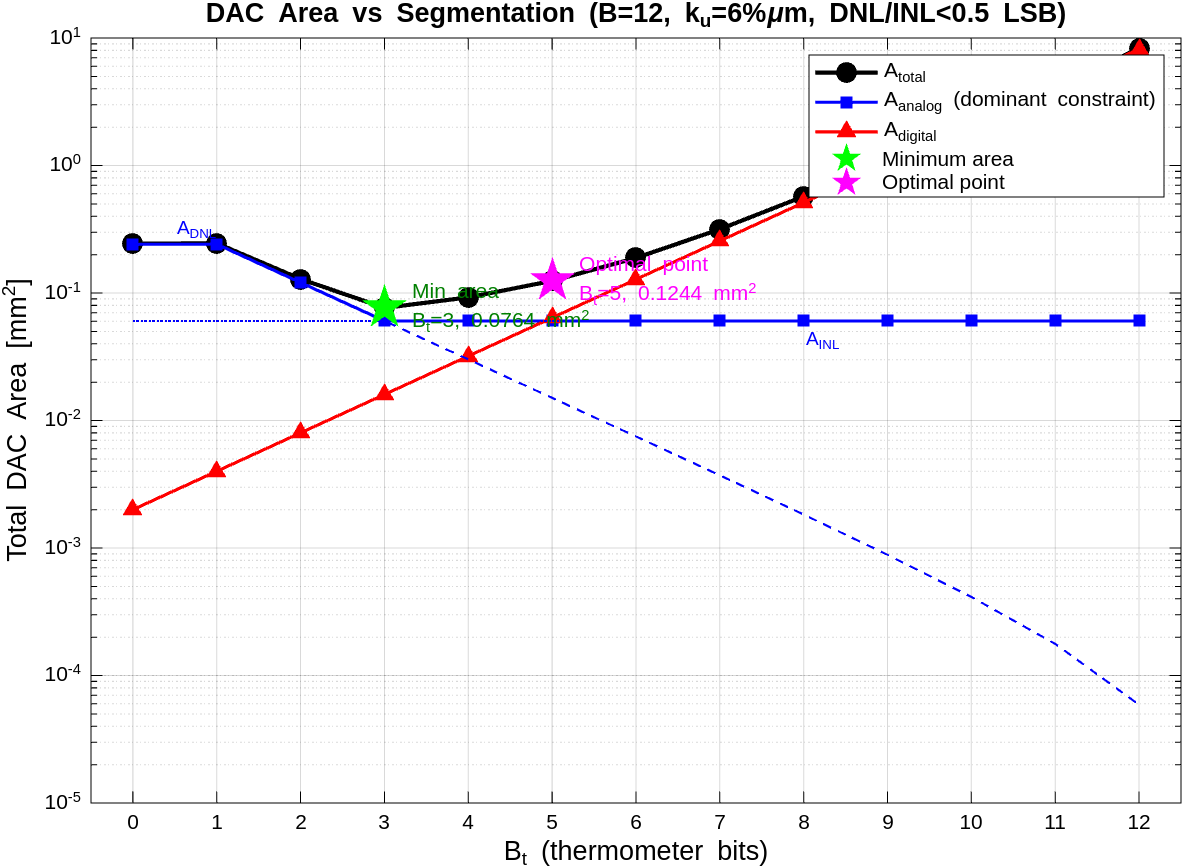
\includegraphics[width=0.9\textwidth]{p3b_area_vs_segmentation.png}
    \caption{Total DAC area vs.\ number of thermometer bits $B_t$. The minimum area occurs at $B_t = 3$ (green), and the optimal point (analog $\approx$ digital) at $B_t = 5$ (magenta).}
    \label{fig:p3b}
\end{figure}

%% ============================================================
%% PROBLEM 4
%% ============================================================
\section{Monte Carlo Simulation}

\textbf{Task:} Simulate the minimum-area design from Problem~3(a)(i) using the provided starter file \texttt{hw2\_dac.m}, add DNL code, and iterate $A_\text{unit}$ to achieve 95\% yield.

\subsection{Part (a): Added DNL Code}

The following code was added to \texttt{hw2\_dac.m} below the \texttt{"Your code goes here"} marker:

\begin{lstlisting}
% calculate dnl
for m=1:r
  avg_width = (code(m, end)-code(m, 1))/(2^B-1);
  dnl(m, :) = diff(code(m,:)) ./ avg_width - 1;
end

% dnl scatter plot
figure(3); clf; hold on;
xlabel('Code');
ylabel('DNL [LSB]');
axis([0 2^B-2 -(dnlspec+0.05) (dnlspec+0.05)]);
line([0 2^B-2], [dnlspec dnlspec]);
line([0 2^B-2], [-dnlspec -dnlspec]);

bad_dacs_dnl=0;
for m=1:r
  figure(3);
  plot(0:2^B-2, dnl(m,:));
  if find(abs(dnl(m,:))>dnlspec)
      bad_dacs_dnl=bad_dacs_dnl+1;
  end
end

figure(3); hold off;
title(sprintf('DNL envelope of %d runs. %d bad DAC(s).', ...
    r, bad_dacs_dnl));

% dnl rms plot
dnl_rms = sqrt(sum( dnl.^2, 1 ) ./r);
[maxdnlrms dmax] = max(dnl_rms);
figure(4);
plot(0:2^B-2, dnl_rms, dmax, maxdnlrms, '*');
xlabel('Code');
ylabel('DNL [LSB]');
title(sprintf('RMS DNL of %d runs. (max=%1.3fLSBrms)', ...
    r, maxdnlrms));
axis([0 2^B-2 0 maxdnlrms+0.01]);
\end{lstlisting}

\subsection{Part (b): Initial Design Plots ($B_t = 3$, $A_\text{unit} = 14.75$\,$\mu$m\textsuperscript{2})}

Using the minimum-area design from Problem~3(a)(i): $B_t = 3$, $A_\text{unit} = 14.75$\,$\mu$m\textsuperscript{2}, $\sigma_u = 0.01562$.

\begin{figure}[H]
    \centering
    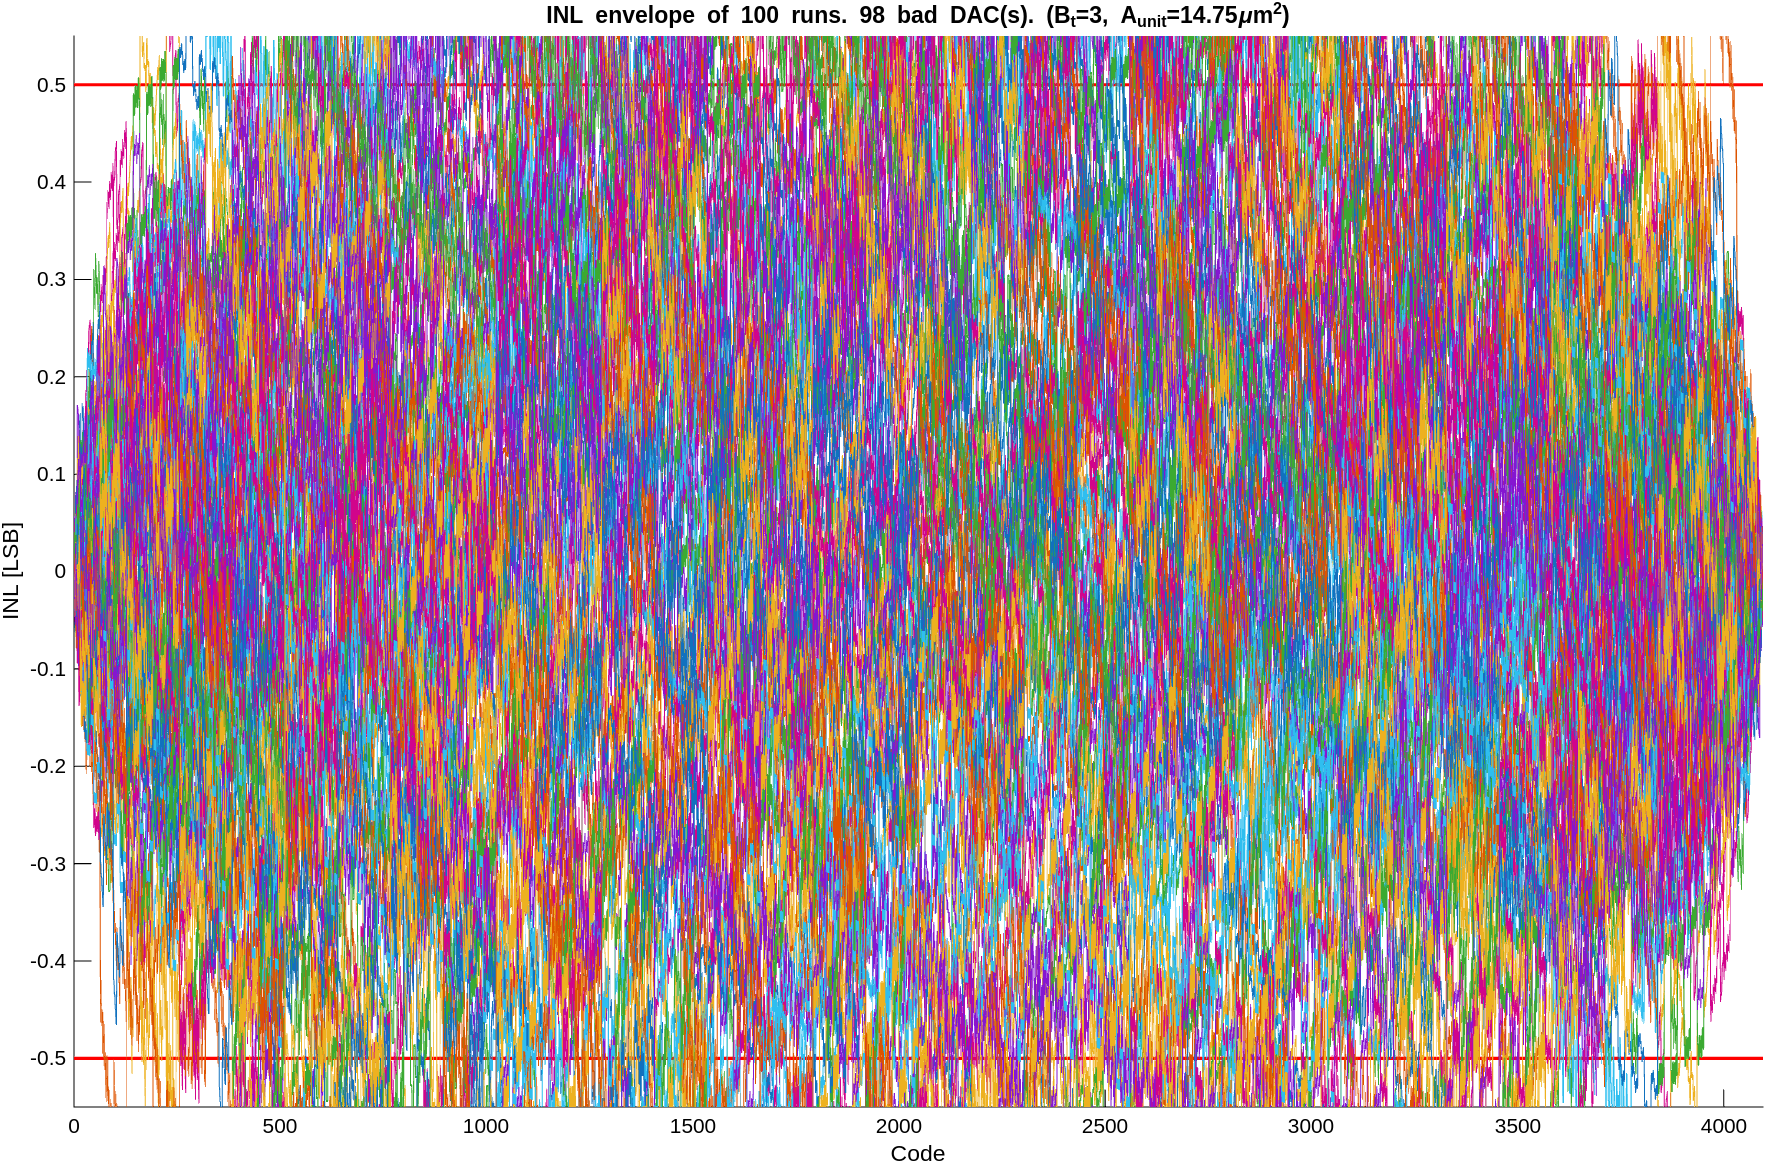
\includegraphics[width=0.85\textwidth]{p4b_inl_envelope_A15.png}
    \caption{INL envelope of 100 Monte Carlo runs ($A_\text{unit} = 14.75$\,$\mu$m\textsuperscript{2}). 98 bad DACs.}
    \label{fig:p4b_inl_env_init}
\end{figure}

\begin{figure}[H]
    \centering
    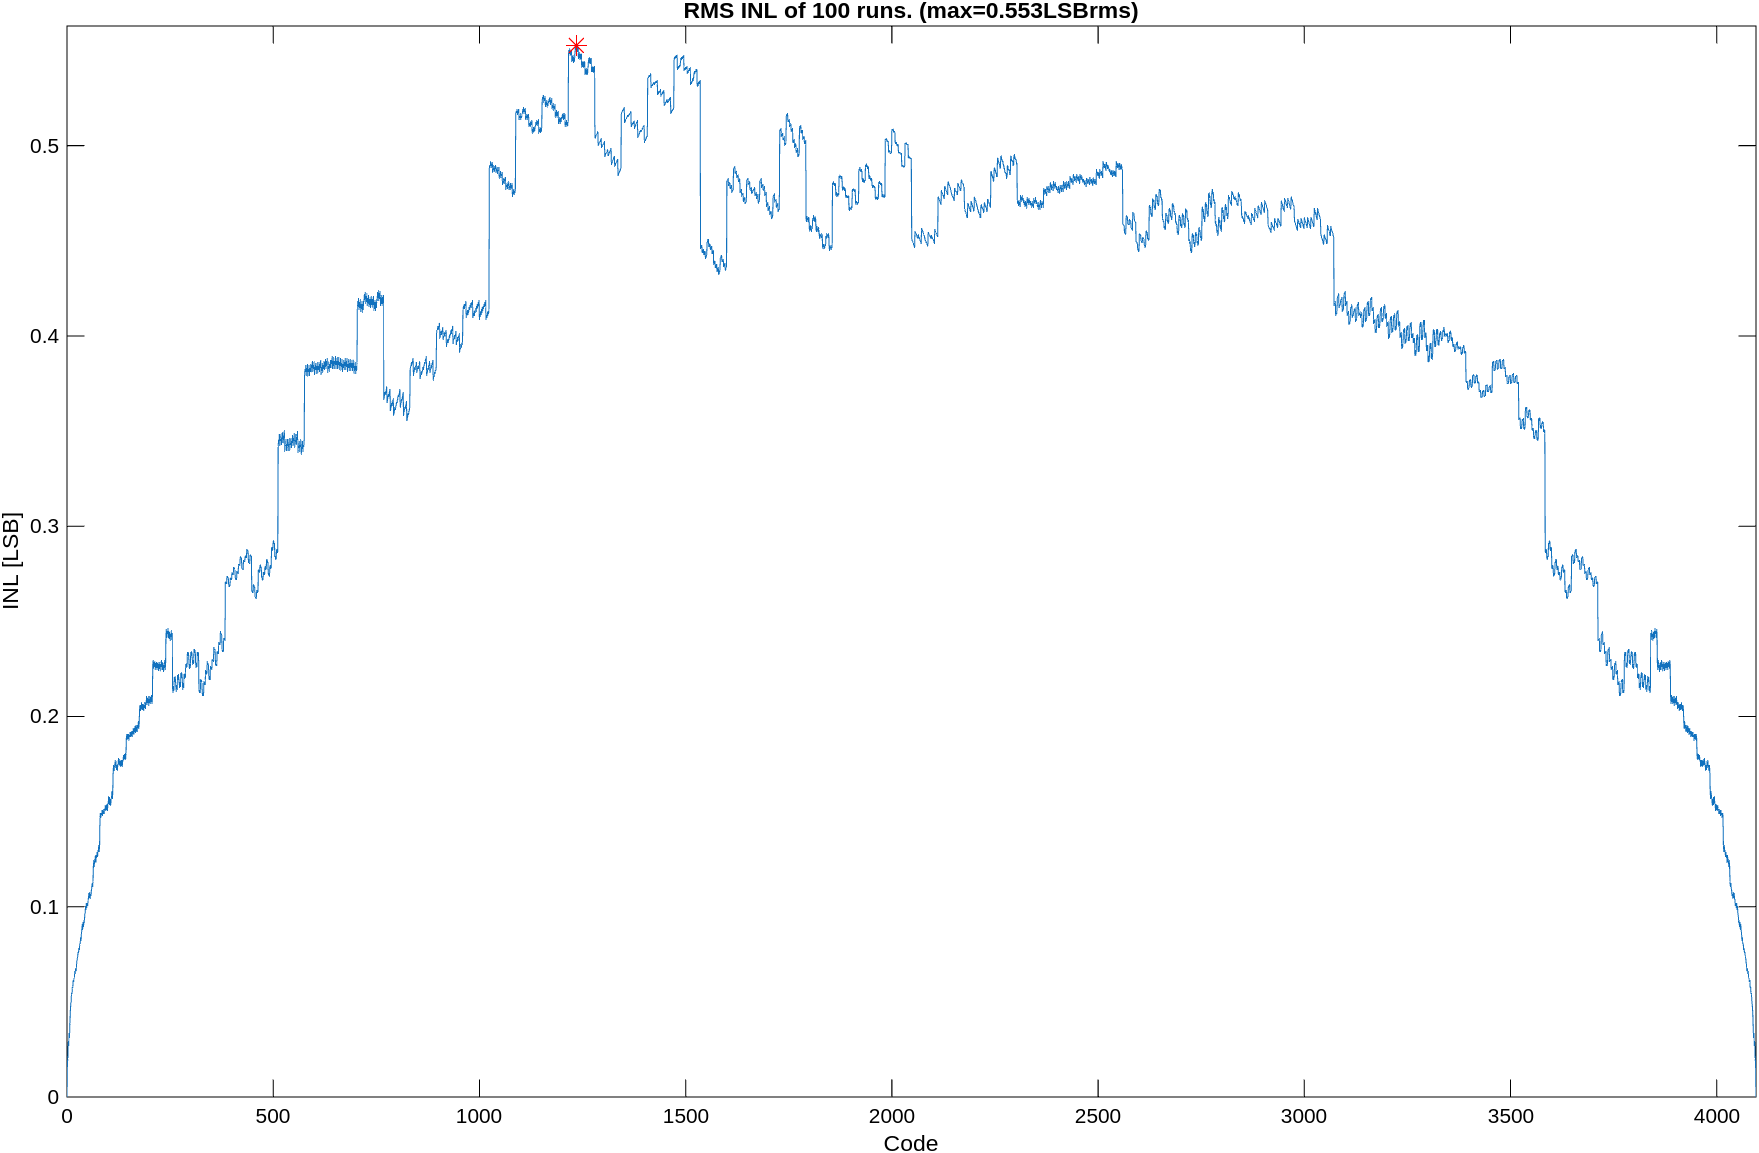
\includegraphics[width=0.85\textwidth]{p4b_inl_rms_A15.png}
    \caption{RMS INL of 100 runs ($A_\text{unit} = 14.75$\,$\mu$m\textsuperscript{2}).}
    \label{fig:p4b_inl_rms_init}
\end{figure}

\begin{figure}[H]
    \centering
    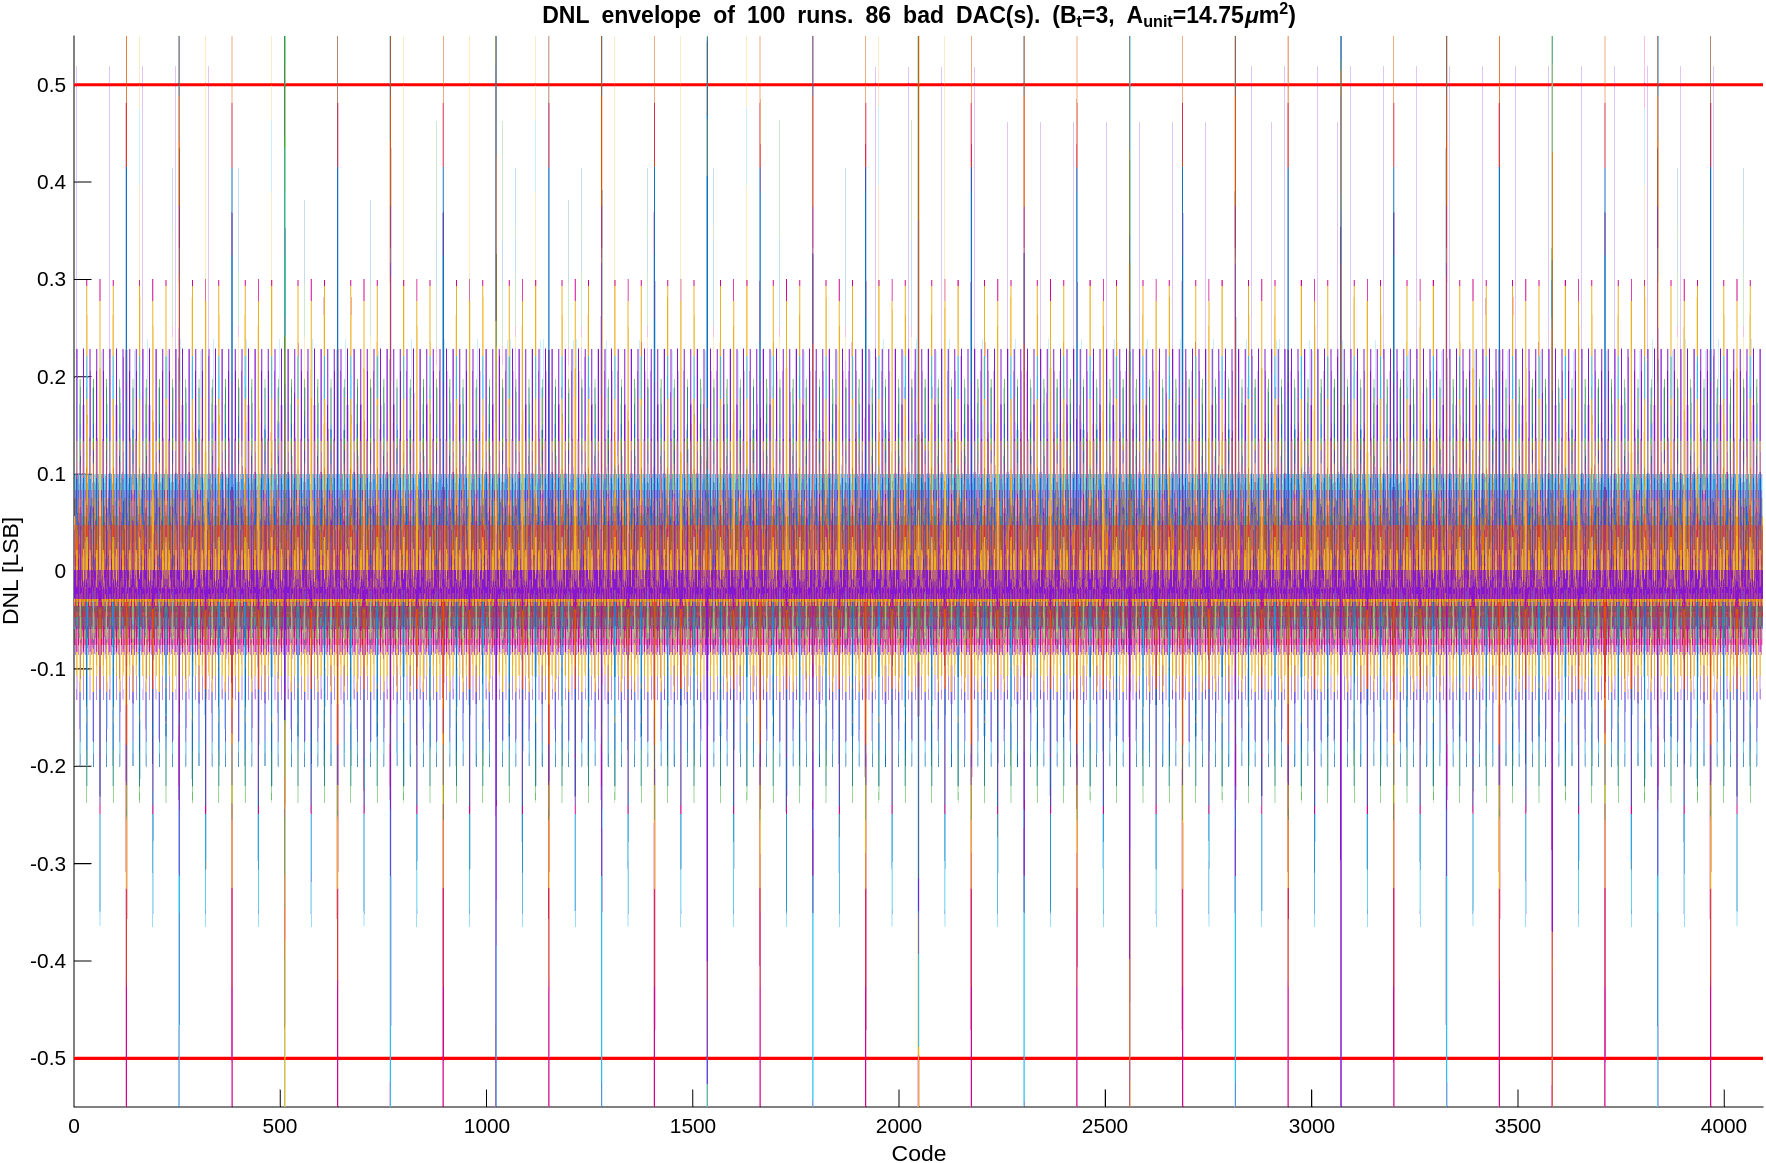
\includegraphics[width=0.85\textwidth]{p4b_dnl_envelope_A15.png}
    \caption{DNL envelope of 100 Monte Carlo runs ($A_\text{unit} = 14.75$\,$\mu$m\textsuperscript{2}). 86 bad DACs.}
    \label{fig:p4b_dnl_env_init}
\end{figure}

\begin{figure}[H]
    \centering
    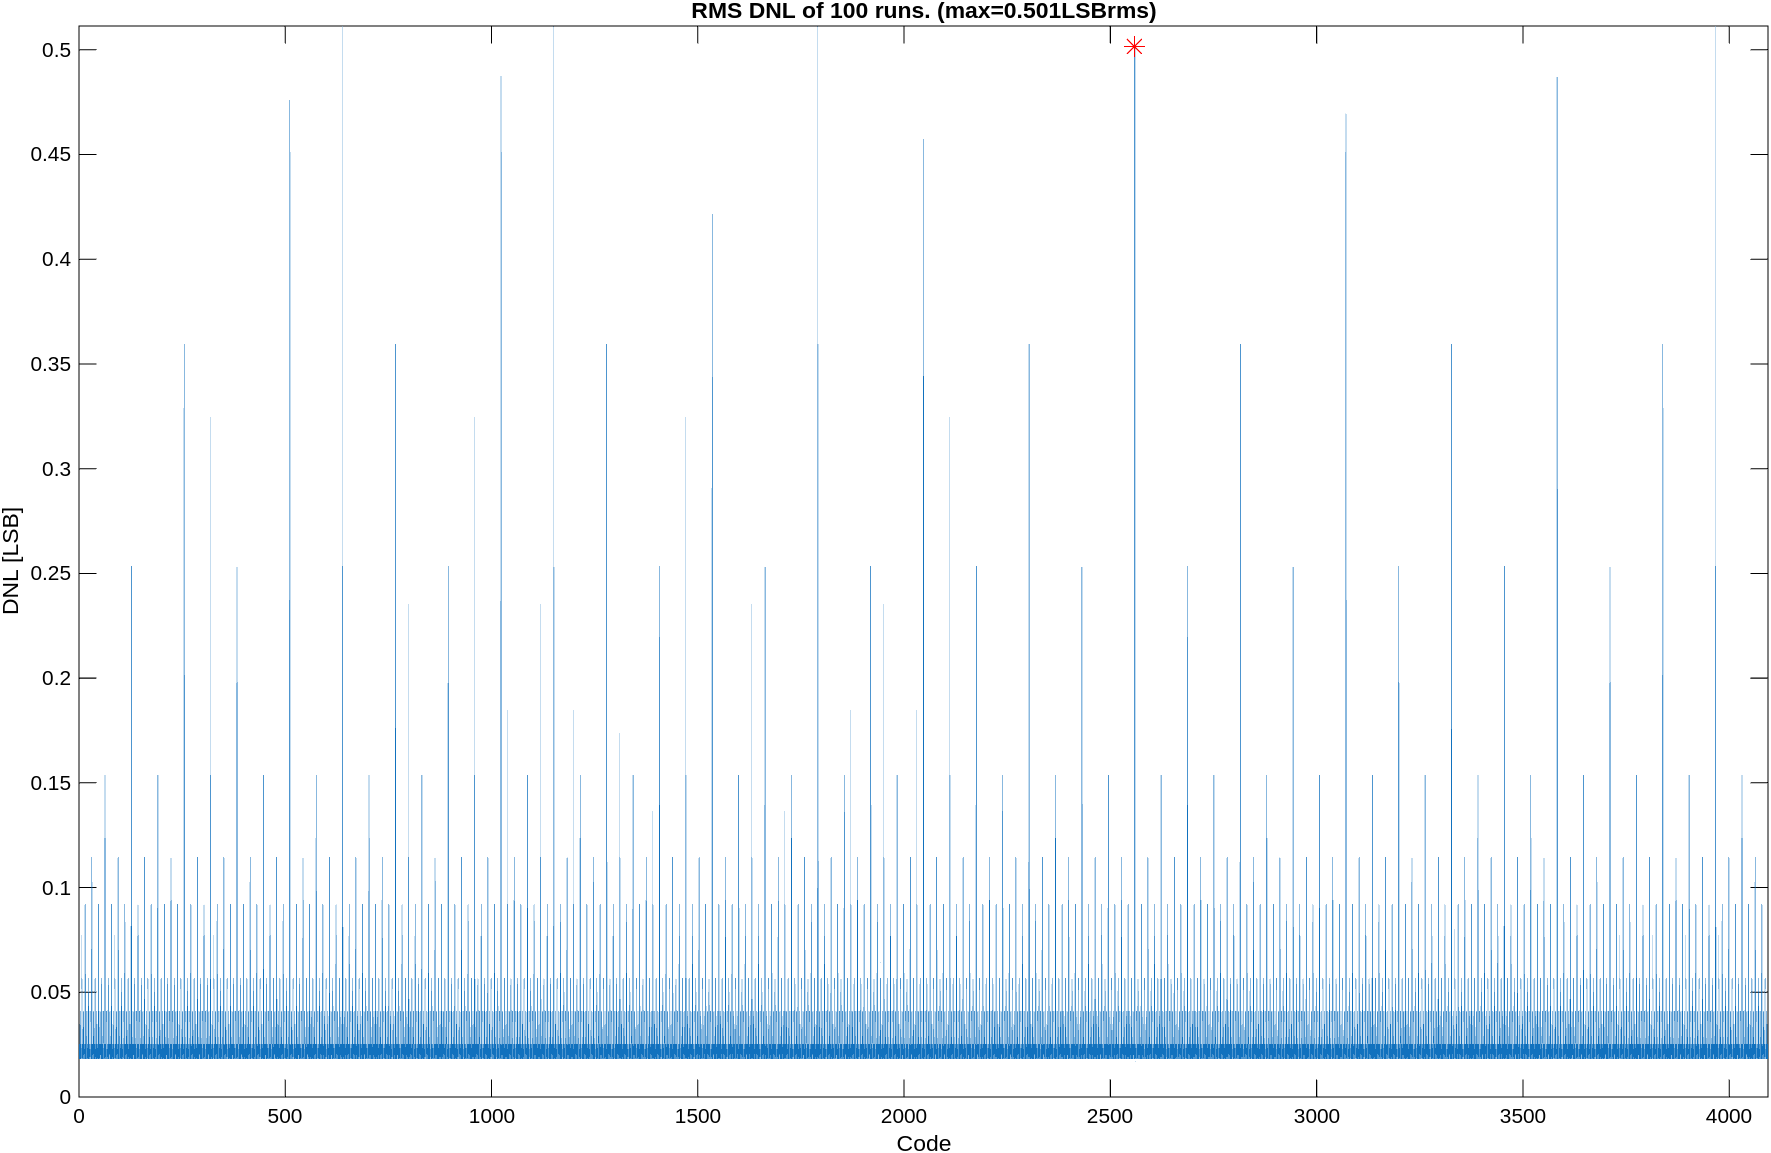
\includegraphics[width=0.85\textwidth]{p4b_dnl_rms_A15.png}
    \caption{RMS DNL of 100 runs ($A_\text{unit} = 14.75$\,$\mu$m\textsuperscript{2}).}
    \label{fig:p4b_dnl_rms_init}
\end{figure}

\textbf{Results:} 98/100 bad INL, 86/100 bad DNL --- yield is only \textbf{1\%}.

\subsection{Part (c): Does the Initial Design Meet the Yield Spec?}

\textbf{No}, the initial design completely fails the 95\% yield target. Only 1 out of 100 DACs meets both DNL $< 0.5$\,LSB and INL $< 0.5$\,LSB simultaneously.

\textbf{Why it fails:} The hand calculation in Problem~3 followed the paper's procedure of setting the spec equal to $1\sigma$ of the worst-case nonlinearity:
\begin{equation}
    \sigma_{\text{INL,max}} = 32\,\sigma_u = 0.5\;\text{LSB} \quad(1\sigma)
\end{equation}

This means the worst-case INL exceeds 0.5\,LSB about 32\% of the time at the most critical code (midscale). With 4096 codes and many contributing to the peak INL, virtually every DAC has at least one code violating the spec.

To achieve 95\% yield across all codes simultaneously, we need $\sim$3$\sigma$ margin, i.e., the spec should equal approximately $3\sigma$ rather than $1\sigma$. This requires $\sigma_u$ to be $\sim$3$\times$ smaller, meaning $A_\text{unit}$ must be $\sim$9$\times$ larger (since $A \propto 1/\sigma^2$).

\subsection{Part (d): Adjusted Design for 95\% Yield}

Sweeping $A_\text{unit}$ from 110 to 180\,$\mu$m\textsuperscript{2} (with $B_t = 3$ fixed), averaging over 10 random seeds:

\begin{table}[H]
\centering
\caption{Yield sweep results (averaged over 10 seeds, 100 runs each).}
\begin{tabular}{@{}ccc@{}}
\toprule
$A_\text{unit}$ ($\mu$m$^2$) & $\sigma_u$ & Average Yield \\
\midrule
110 & 0.00572 & 89.7\% \\
120 & 0.00548 & 91.8\% \\
130 & 0.00526 & 93.7\% \\
\textbf{140} & \textbf{0.00507} & \textbf{95.5\%} \\
150 & 0.00490 & 96.1\% \\
160 & 0.00474 & 97.2\% \\
\bottomrule
\end{tabular}
\label{tab:yield_sweep}
\end{table}

$\mathbf{A_\text{unit} = 140}$\,$\mu$\textbf{m}\textsuperscript{\textbf{2}} achieves an average yield of \textbf{95.5\%} ($\leq 5$ bad DACs on average out of 100), meeting the spec.

\subsubsection{Final Design}

\begin{table}[H]
\centering
\caption{Final DAC design parameters.}
\begin{tabular}{@{}ll@{}}
\toprule
Parameter & Value \\
\midrule
$B_t$ & 3 \\
$B_b$ & 9 \\
$A_\text{unit}$ & 140\,$\mu$m\textsuperscript{2} \\
$\sigma_u$ & 0.00507 \\
$A_\text{analog}$ & $4096 \times 140 = 573{,}440$\,$\mu$m\textsuperscript{2} \\
$A_\text{digital}$ & $8 \times 2000 = 16{,}000$\,$\mu$m\textsuperscript{2} \\
\midrule
$\mathbf{A_\text{total}}$ & $\mathbf{589{,}440}$\,$\mu$\textbf{m}\textsuperscript{\textbf{2}} $\mathbf{= 0.589}$\,\textbf{mm}\textsuperscript{\textbf{2}} \\
\bottomrule
\end{tabular}
\end{table}

The final area is about 7.7$\times$ larger than the 1$\sigma$ minimum-area design (0.076\,mm\textsuperscript{2}). The $\sim$9.5$\times$ increase in unit element area corresponds to a $\sqrt{9.5} \approx 3.1\times$ reduction in $\sigma_u$, confirming that $\sim$3$\sigma$ margin is needed for 95\% yield with a 12-bit DAC.

\subsubsection{Final Plots ($B_t = 3$, $A_\text{unit} = 140$\,$\mu$m\textsuperscript{2})}

\begin{figure}[H]
    \centering
    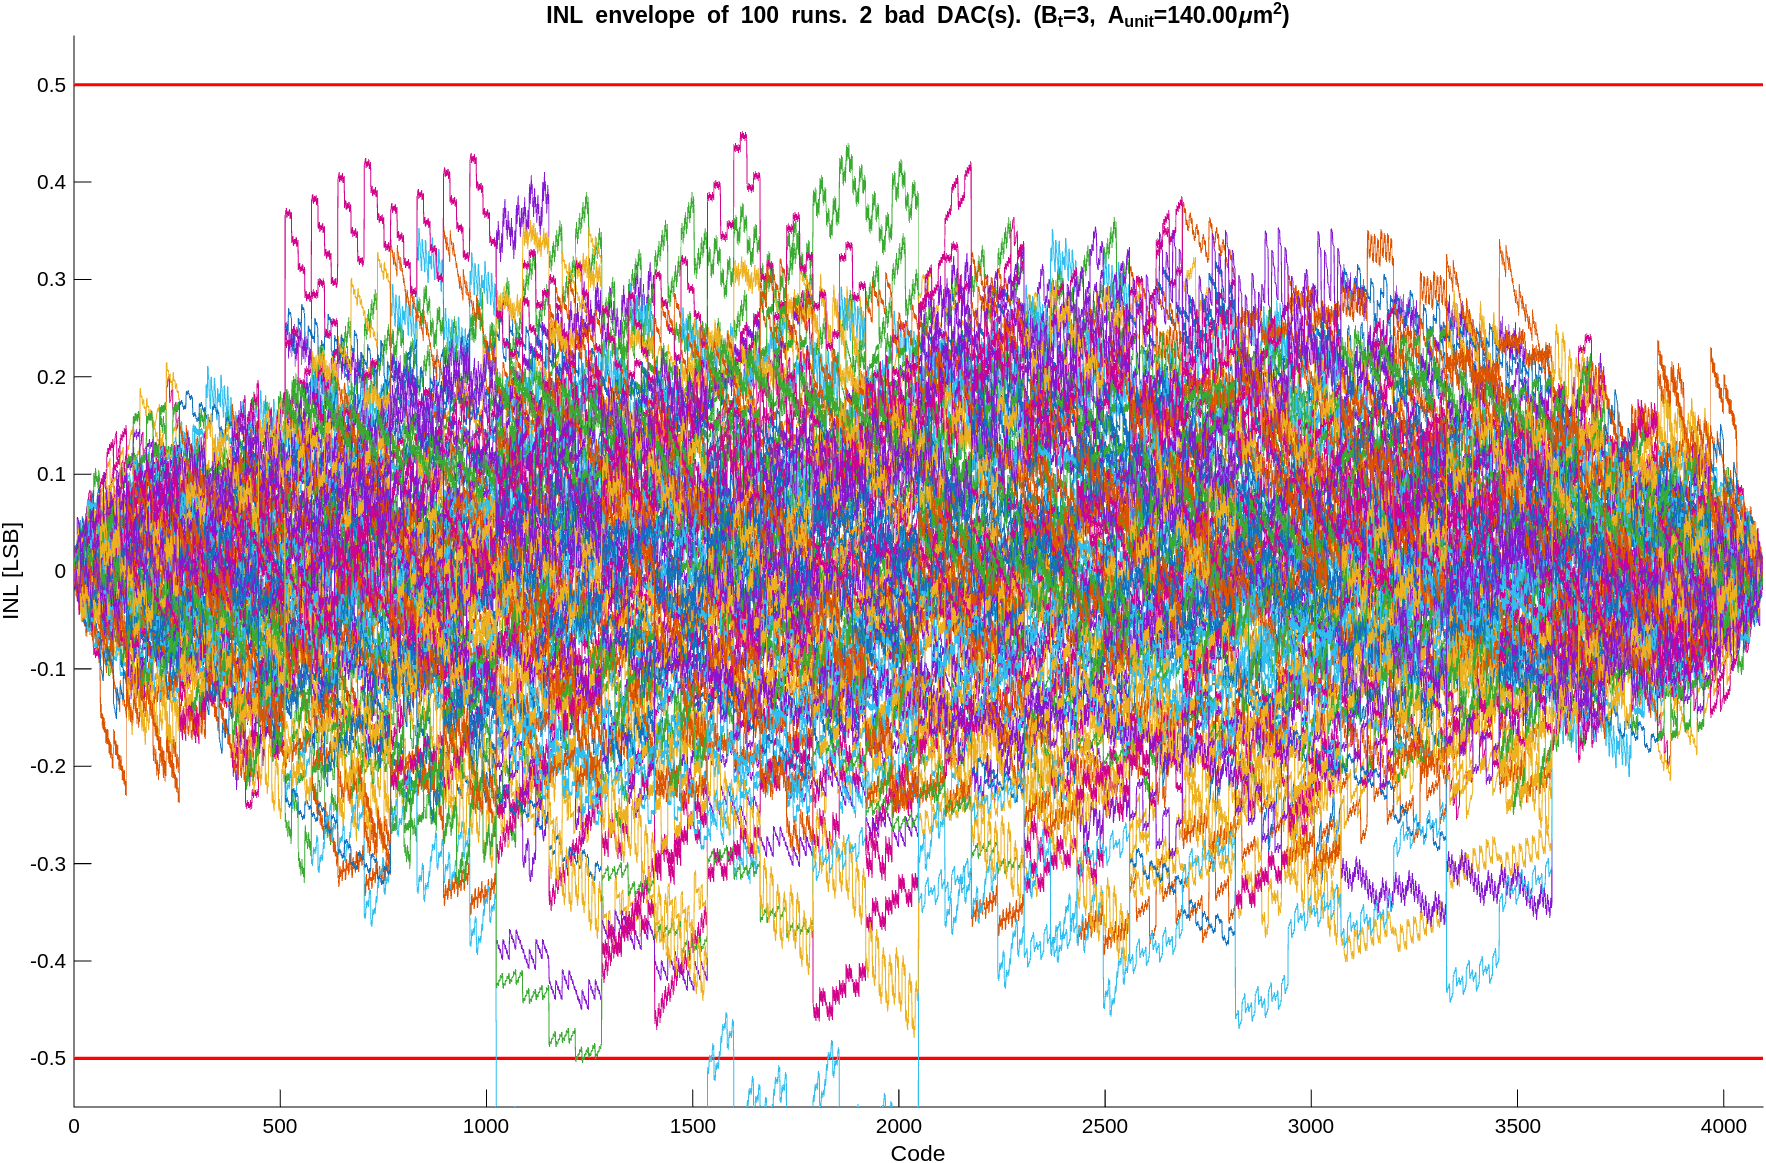
\includegraphics[width=0.85\textwidth]{p4b_inl_envelope_A140.png}
    \caption{INL envelope of 100 Monte Carlo runs ($A_\text{unit} = 140$\,$\mu$m\textsuperscript{2}). 2 bad DACs.}
    \label{fig:p4d_inl_env}
\end{figure}

\begin{figure}[H]
    \centering
    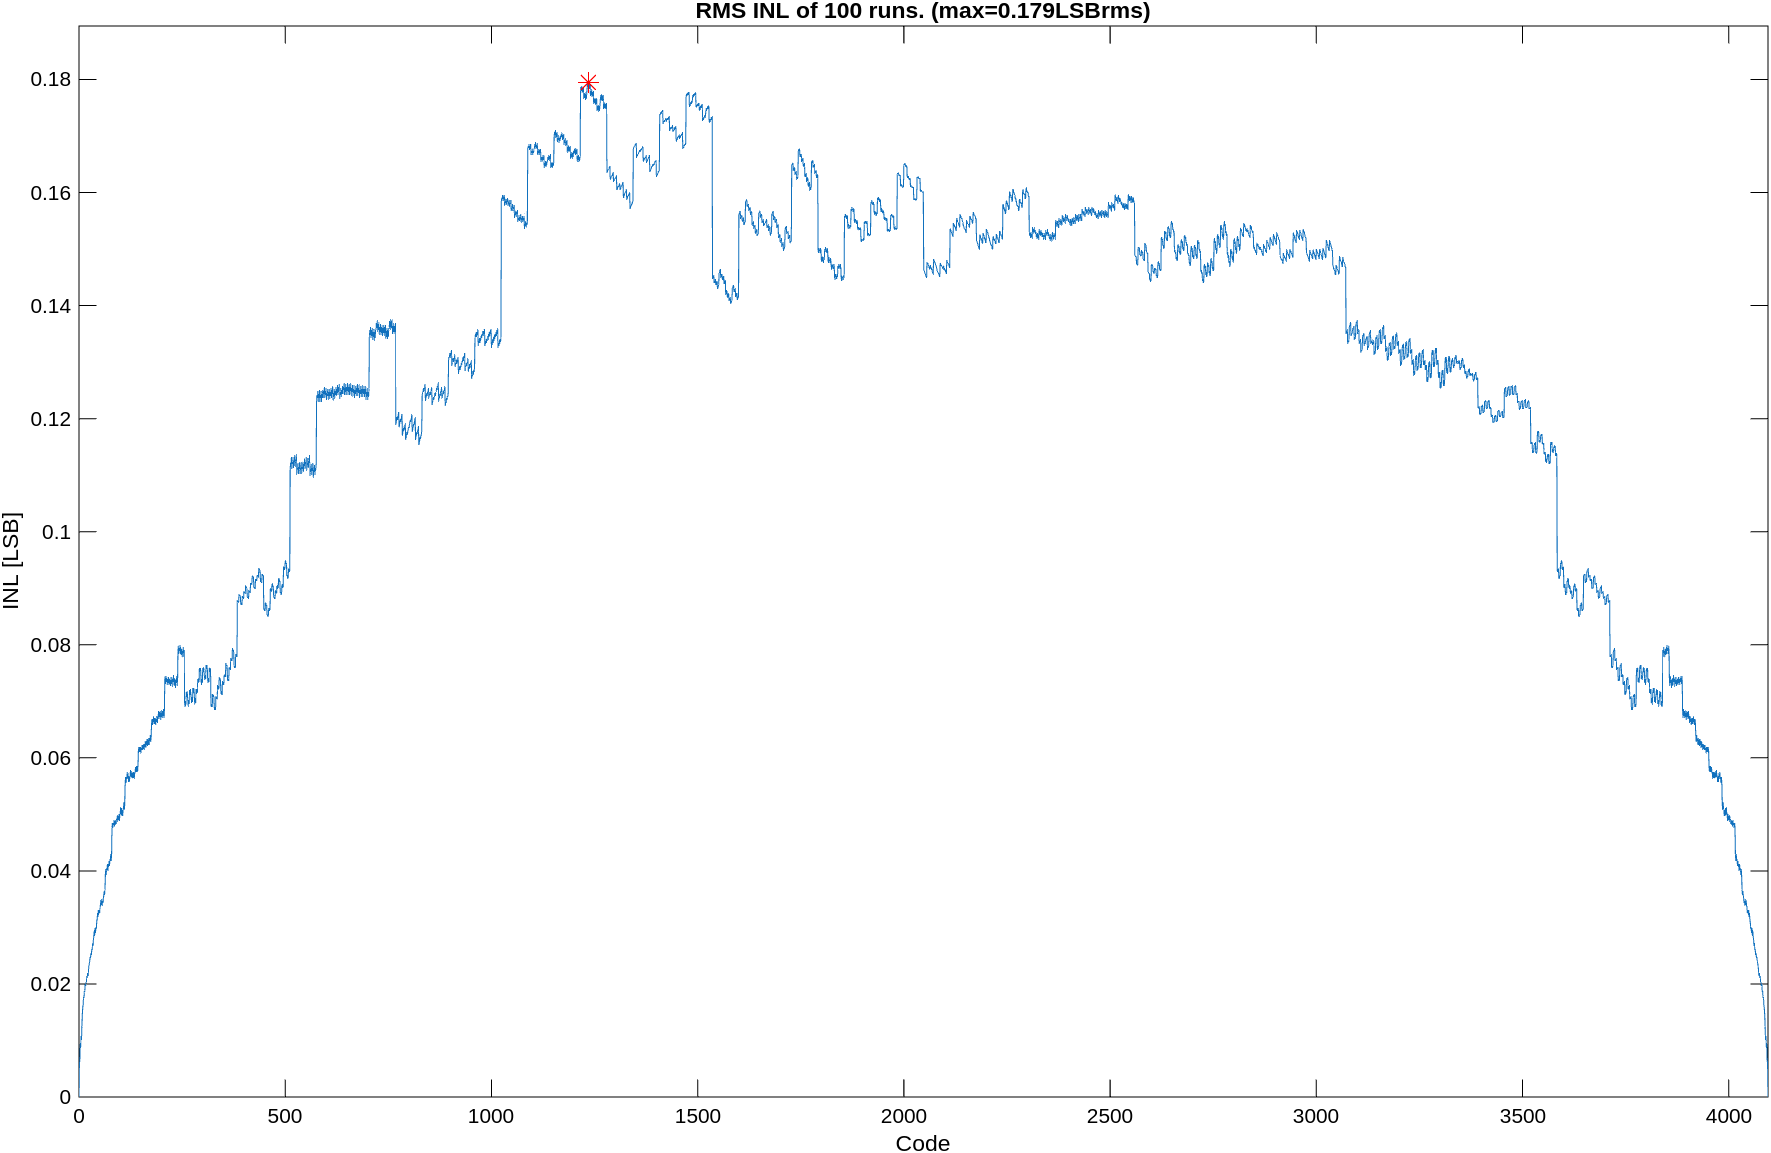
\includegraphics[width=0.85\textwidth]{p4b_inl_rms_A140.png}
    \caption{RMS INL of 100 runs ($A_\text{unit} = 140$\,$\mu$m\textsuperscript{2}). Peak = 0.179\,LSBrms at midcode.}
    \label{fig:p4d_inl_rms}
\end{figure}

\begin{figure}[H]
    \centering
    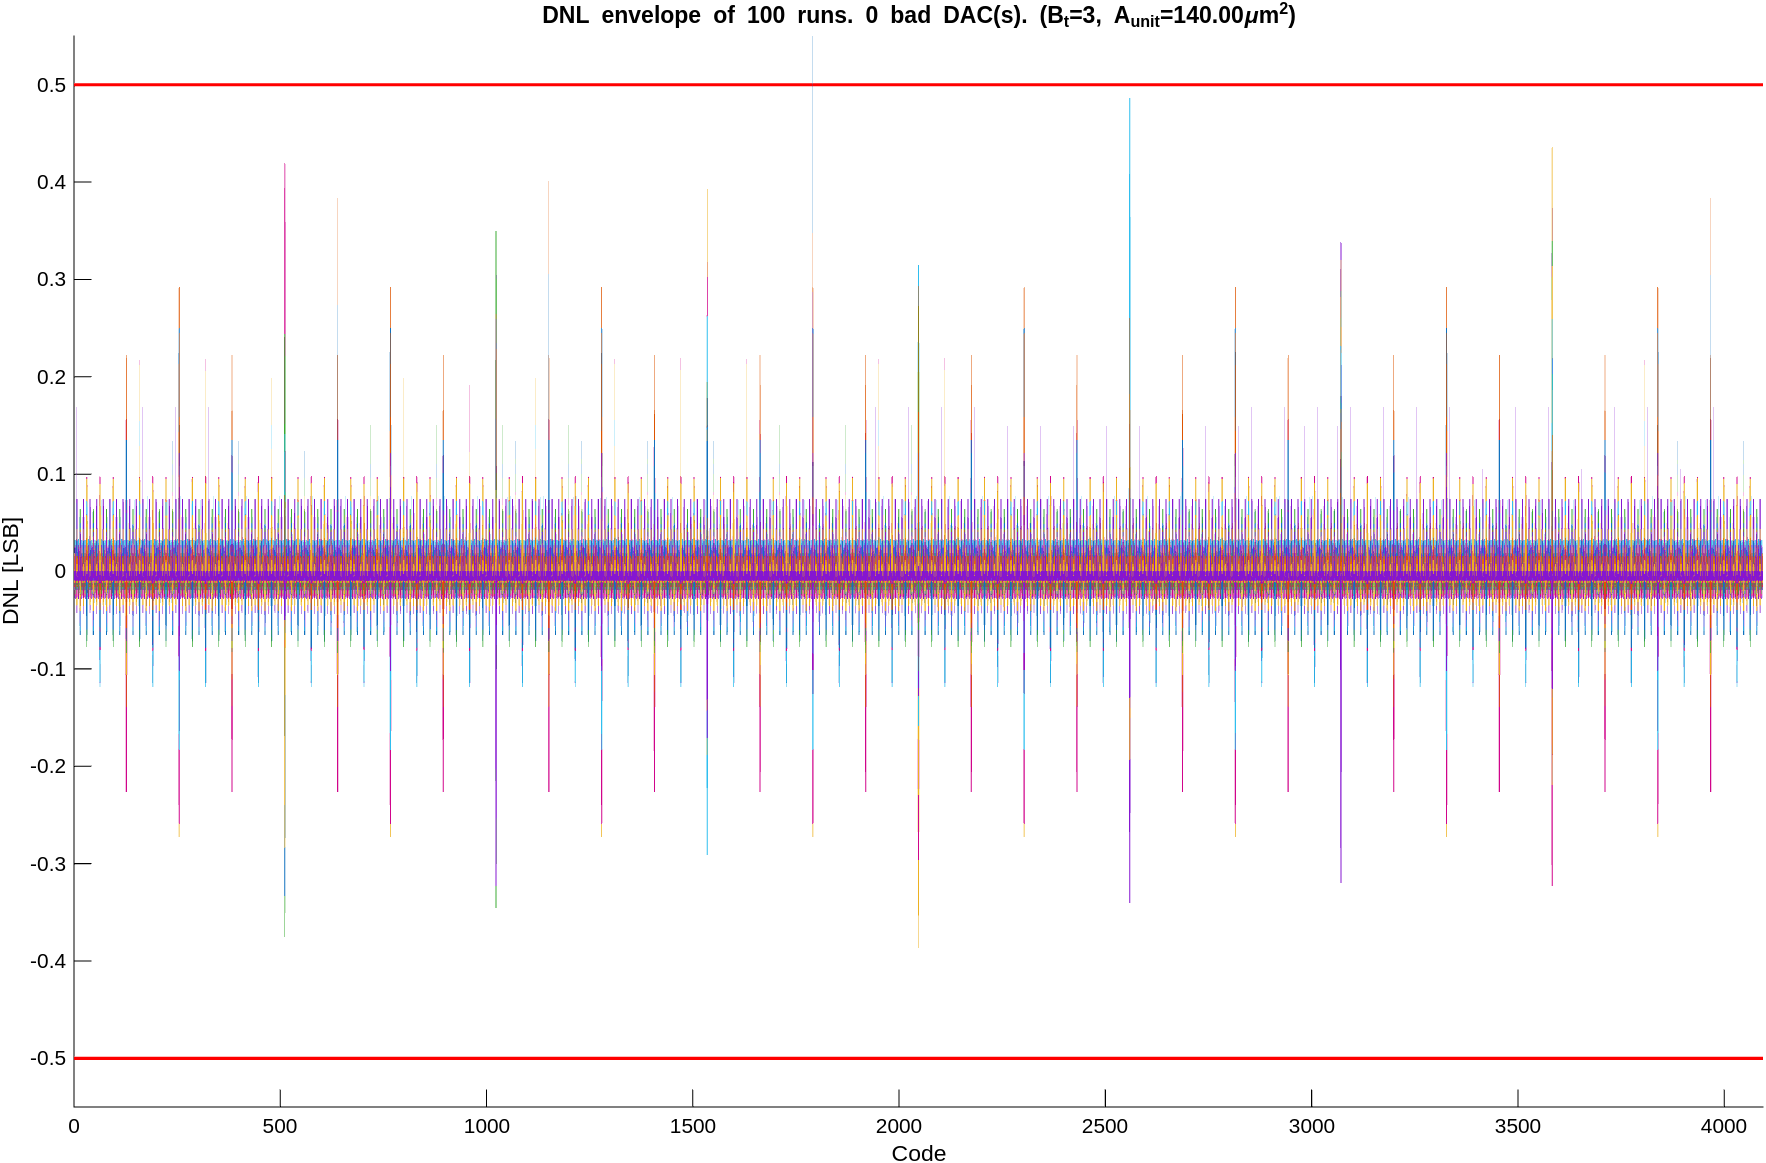
\includegraphics[width=0.85\textwidth]{p4b_dnl_envelope_A140.png}
    \caption{DNL envelope of 100 Monte Carlo runs ($A_\text{unit} = 140$\,$\mu$m\textsuperscript{2}). 0 bad DACs.}
    \label{fig:p4d_dnl_env}
\end{figure}

\begin{figure}[H]
    \centering
    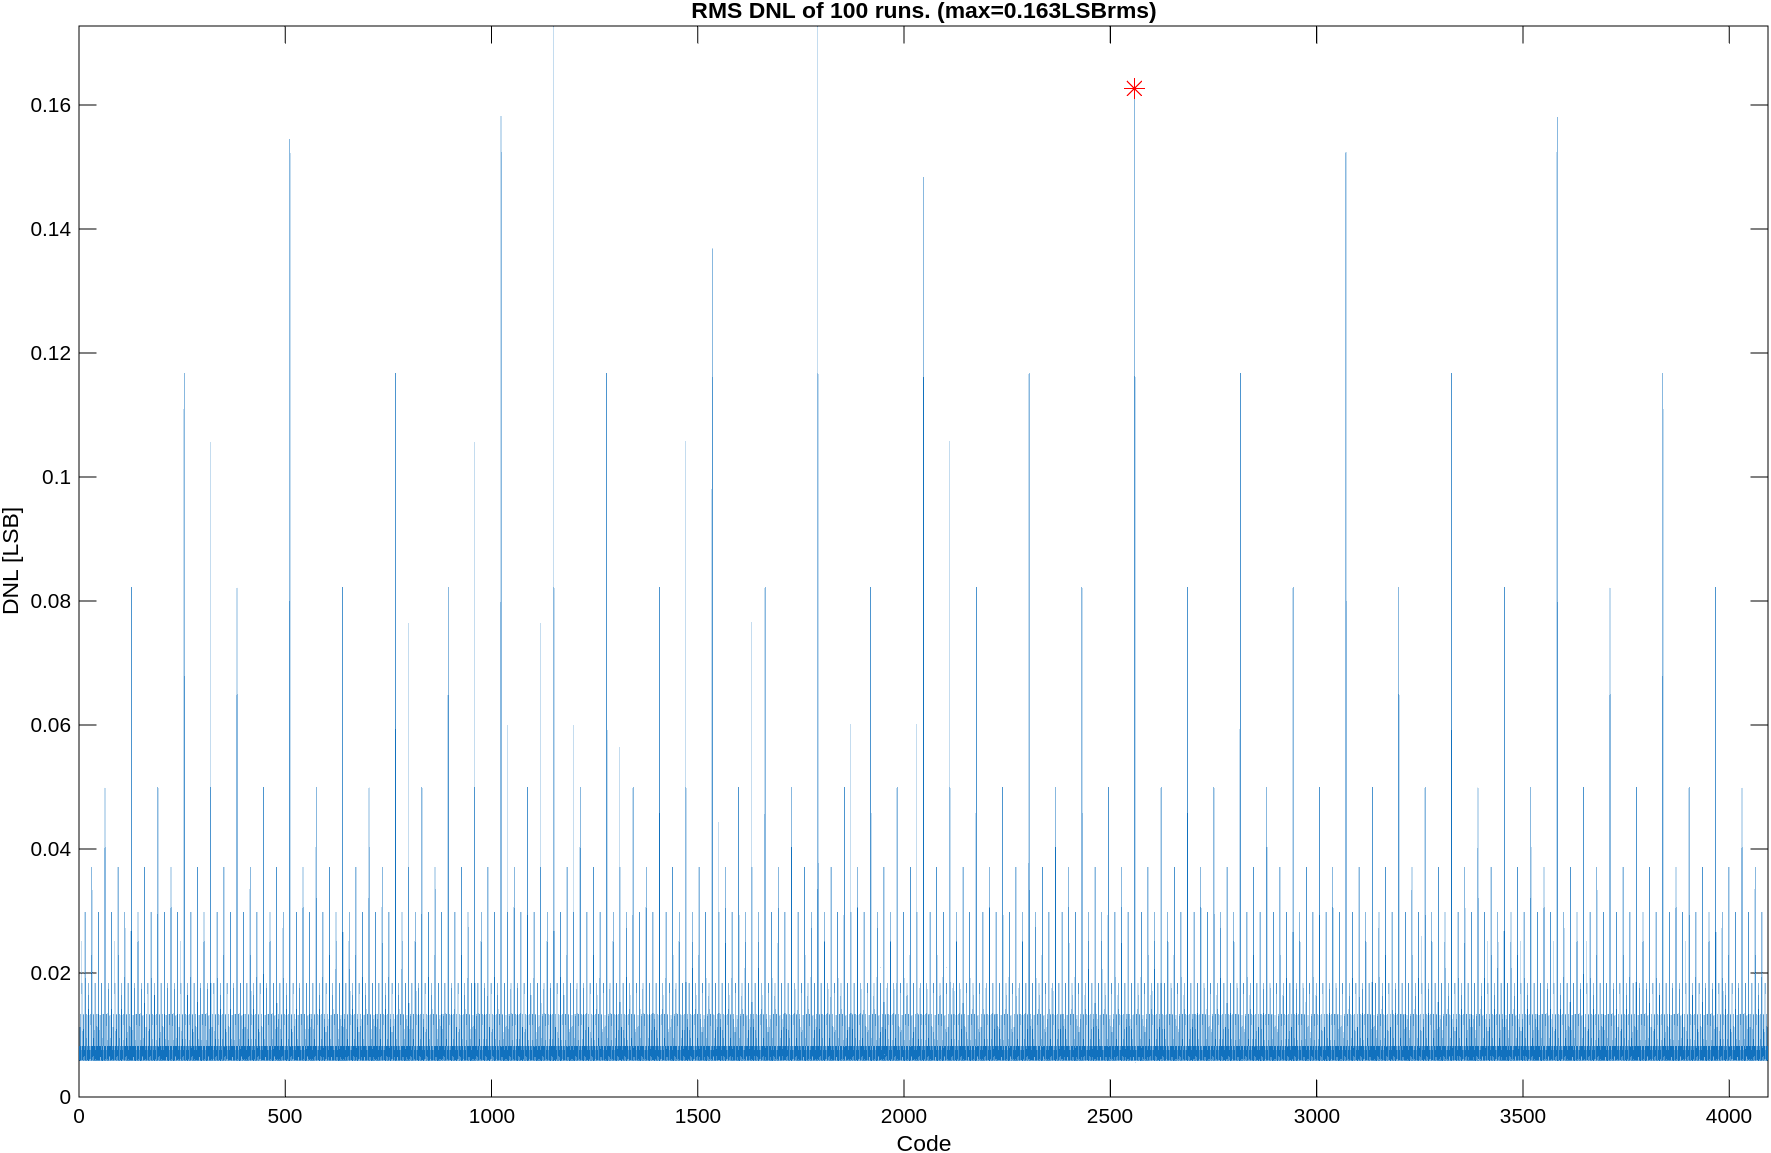
\includegraphics[width=0.85\textwidth]{p4b_dnl_rms_A140.png}
    \caption{RMS DNL of 100 runs ($A_\text{unit} = 140$\,$\mu$m\textsuperscript{2}). Peak = 0.163\,LSBrms at major carry transitions.}
    \label{fig:p4d_dnl_rms}
\end{figure}

\textbf{Final results:} Bad INL: 2/100, Bad DNL: 0/100, Overall yield: \textbf{98\%} --- meets the 95\% target.

\end{document}
